\chapter{Experimental Results}
\label{ch:results}

Each section restates the query and index configurations, then separates the observed latency from its plan explanation and cost. All reported measurements come from the Phase 8 accepted evidence. A, B, and C are compared only within the same DBMS and query.

\section{UC1: Compound B-Tree Index (100K Rows)}

\ReportBlock{Experimental Setup}
On 100K catalog rows, U1a filters by all three keys; U1b by \texttt{OWNER, OBJECT\_TYPE}; U1c omits the leading \texttt{OWNER}; U1d filters by \texttt{OWNER} and sorts by the other two keys. A has no optional index, B indexes \texttt{OWNER}, and C indexes \texttt{(OWNER, OBJECT\_TYPE, OBJECT\_ID)}. C should help aligned filters and sort order; a common owner, a missing leading key, or many base-row lookups can defeat it.

\ReportBlock{Measured Results}
Table~\ref{tab:uc1-read} and Figure~\ref{fig:uc1} show the median read latencies and physical work across the four UC1 queries.

\begin{table}[H]
\centering\small
\caption{UC1: explicit A/B/C read medians and C's selected physical work.}
\label{tab:uc1-read}
\begin{tabularx}{\linewidth}{@{}l l r r r >{\raggedright\arraybackslash}X@{}}
\toprule
Engine & Query & A p50 (ms) & B p50 (ms) & C p50 (ms) & Work in C\\
\midrule
SQL & U1a full key & 32.36 & 24.53 & 9.46 & 5 page reads (seek)\\
SQL & U1b prefix & 104.48 & 84.29 & 97.99 & 2,730 pages (scan)\\
SQL & U1c no leading key & 37.01 & 31.97 & 20.04 & 657 pages (index scan)\\
SQL & U1d sorted & 38.02 & 11.12 & 10.52 & 405 pages; no Sort\\
\midrule
Mongo & U1a full key & 241.03 & 462.78 & 2.34 & 2 documents examined\\
Mongo & U1b prefix & 253.16 & 457.73 & 39.31 & 3,405 documents\\
Mongo & U1c no leading key & 228.33 & 204.50 & 232.18 & 100K documents (scan)\\
Mongo & U1d sorted & 236.43 & 10.04 & 7.97 & 398 documents; no Sort\\
\bottomrule
\end{tabularx}
\par\smallskip\scriptsize\raggedright Ratios discussed below compare configurations within one engine. SQL work counts logical 8 KB pages; Mongo work counts documents.\par
\end{table}

\begin{figure}[H]
\centering
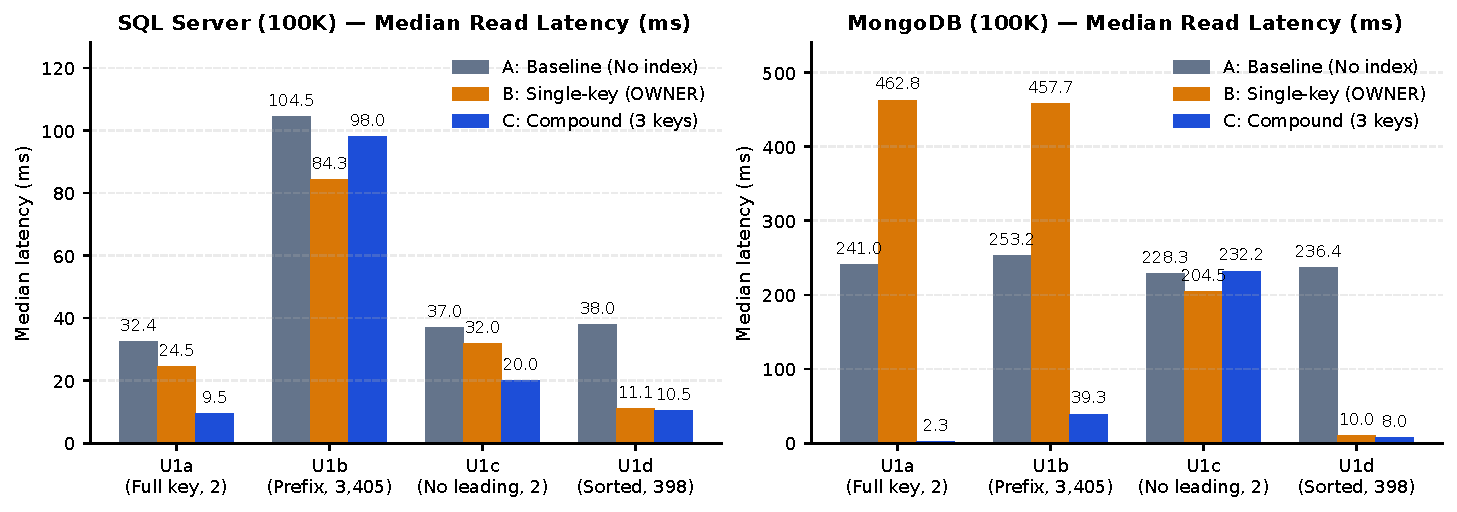
\includegraphics[width=0.94\linewidth]{figures/fig_uc1_compound.pdf}
\caption{UC1 (100K) median read latency. In MongoDB (right), Single-Key B on \texttt{OWNER='SYS'} is slower than an unindexed scan on U1a/U1b, whereas Compound C cuts U1a latency to $2.3$\,ms.}
\label{fig:uc1}
\end{figure}

\ReportBlock{Why These Results Occurred}
Three important physical behaviors explain the numbers in Table~\ref{tab:uc1-read}:
\begin{enumerate}
\item \textbf{Single-Key B Regression on Skewed Data (\texttt{U1a}, \texttt{U1b}):} Because \texttt{OWNER = 'SYS'} matches $71,802$ of the $100,000$ rows, SQL Server's cost-based optimizer refuses to use Index B on \texttt{U1a} and \texttt{U1b}, choosing a sequential $2,730$-page \texttt{Table Scan}. MongoDB, however, chooses \texttt{ix\_uc1\_owner} and performs $71,802$ random document fetches (\texttt{IXSCAN + FETCH}), making Config B \textbf{nearly $2\times$ slower than having no index at all} ($462.78$\,ms vs.\ $241.03$\,ms). Compound Index C fixes this by narrowing the seek to all three columns ($2$ examined docs in MongoDB; $5$ page reads in SQL Server).
\item \textbf{Why SQL Server Skips C on \texttt{U1b} and Why \texttt{U1c} Fails to Seek:} On \texttt{U1b} ($3,405$ matching rows), MongoDB C uses \texttt{IXSCAN + FETCH} ($6.44\times$ faster than A). However, SQL Server C still chooses a $2,730$-page \texttt{Table Scan} (with high tail variance, p95 = $673.3$\,ms) because performing $3,405$ random \texttt{RID Lookup} jumps to the heap costs more I/O than reading the $2,730$ heap pages sequentially. On \texttt{U1c} (which omits the leading column \texttt{OWNER}), neither engine can perform a B-tree seek: MongoDB C falls back to a full \texttt{COLLSCAN}, while SQL Server C scans all $657$ leaf pages of the narrower index (\texttt{Index Scan}) before doing $2$ \texttt{RID Lookup}s.
\item \textbf{Sort Elimination (\texttt{U1d}):} On \texttt{U1d} (\texttt{OWNER = 'CTXSYS' ORDER BY OBJECT\_TYPE, OBJECT\_ID}, $398$ rows), both B and C seek the $398$ rows, but B must run an explicit blocking \texttt{Sort}/\texttt{SORT} operator. Config C reads leaf entries already ordered by \texttt{(OBJECT\_TYPE, OBJECT\_ID)}, eliminating the sort operator and cutting SQL Server p95 latency from $56.56$\,ms in B to $29.11$\,ms in C (and MongoDB p95 from $14.05$\,ms to $8.95$\,ms).
\end{enumerate}

\ReportBlock{Index Cost and Trade-Offs}
As shown in Table~\ref{tab:uc1-tradeoff}, adding two more key columns nearly doubles index storage ($+96.5\%$ in SQL Server; $+87.8\%$ in MongoDB) and reduces MongoDB batch \texttt{INSERT} throughput by $33.5\%$ compared to Baseline A. (In SQL Server, Config A ran first on a freshly created table and paid initial file-allocation overhead, so its $6,148$\,rows/s insert rate reflects cold allocation rather than faster unindexed writes).

\begin{table}[H]
\centering\small
\caption{UC1: index size, build time, and batch insert throughput.}
\label{tab:uc1-tradeoff}
\begin{tabular}{@{}l l r r r@{}}
\toprule
Engine & Index & Size (MiB) & Build (ms) & Insert (rows/s)\\
\midrule
SQL & A: none & 0 & 0 & 6,148$^*$\\
SQL & B: owner & 2.64 & 236 & 17,698\\
SQL & C: compound & 5.19 & 1,969 & 18,393\\
\midrule
Mongo & A: none & 0 & 0 & 39,368\\
Mongo & B: owner & 0.48 & 879 & 28,438\\
Mongo & C: compound & 0.90 & 931 & 26,191\\
\bottomrule
\end{tabular}
\par\smallskip\scriptsize\raggedright $^*$SQL A ran first and incurred initial file-growth overhead; its insert result is not a clean index-maintenance estimate. SQL updates also searched an unindexed ID.\par
\end{table}

\ReportBlock{Practical Verdict}
Use a \textbf{Compound B-Tree Index} when queries consistently filter by the leading column(s) or sort in the exact key order (\texttt{U1a}, \texttt{U1d}). Do \emph{not} expect it to seek when queries omit the leading column (\texttt{U1c}), and remember that if a prefix matches thousands of rows (\texttt{U1b}), SQL Server may still scan the table unless the index also covers the selected columns.

\FloatBarrier
\section{UC2: Filtered and Partial Indexes (100K and 1M Rows)}

\ReportBlock{Experimental Setup}
At 100K and 1M rows, the same type and ID range is queried once for rare \texttt{TEMPORARY='Y'} and once for common \texttt{'N'}. A has no optional index, B indexes all rows, and C indexes only \texttt{'Y'} rows. Expect a small, fast C for Y; C cannot provide a complete access path for N or an unsafe parameterized predicate.

\ReportBlock{Measured Results}
Table~\ref{tab:uc2-read} and Figure~\ref{fig:uc2} present the read performance across both 100K and 1M rows.

\begin{table}[H]
\centering\small
\caption{UC2: Y benefits from subset membership; N cannot use C as a complete path.}
\label{tab:uc2-read}
\begin{tabularx}{\linewidth}{@{}l l r r r r >{\raggedright\arraybackslash}X@{}}
\toprule
Engine / scale & Query & A p50 & B p50 & C p50 & B/C & Work in C\\
\midrule
SQL 100K & Y (82) & 30.66 & 3.05 & 1.00 & 3.04$\times$ & 3 page reads\\
SQL 100K & N (2,108) & 52.67 & 19.38 & 52.72 & 0.37$\times$ & 2,732 pages; scan\\
SQL 1M & Y (615) & 92.32 & 9.00 & 5.99 & 1.50$\times$ & 6 page reads\\
SQL 1M & N (15,810) & 347.95 & 292.28 & 349.62 & 0.84$\times$ & 28,032 pages; scan\\
\midrule
Mongo 100K & Y (82) & 238.95 & 8.82 & 2.24 & 3.94$\times$ & 83 keys\\
Mongo 100K & N (2,108) & 263.78 & 21.98 & 256.30 & 0.09$\times$ & 100K docs; scan\\
Mongo 1M & Y (615) & 2,418.94 & 17.17 & 6.13 & 2.80$\times$ & 616 keys\\
Mongo 1M & N (15,810) & 2,447.95 & 69.45 & 2,438.73 & 0.03$\times$ & 1M docs; scan\\
\bottomrule
\end{tabularx}
\par\smallskip\scriptsize\raggedright All p50 values are milliseconds. B/C is the benefit of C over the full index B for the same query.\par
\end{table}

\begin{figure}[H]
\centering
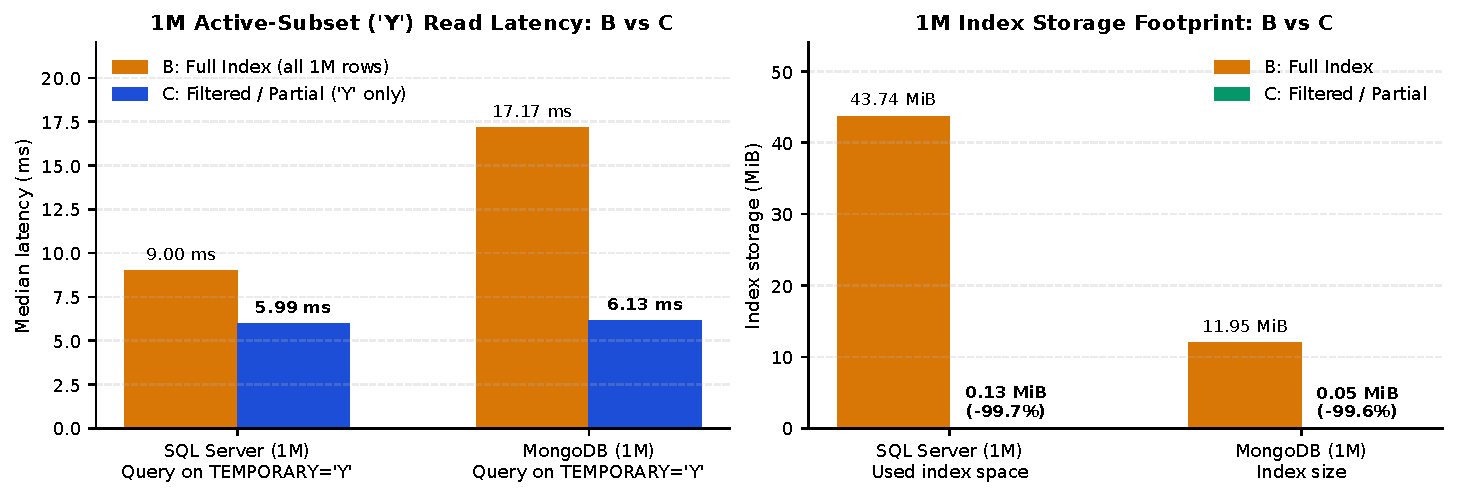
\includegraphics[width=0.94\linewidth]{figures/fig_uc2_filtered.pdf}
\caption{UC2 (1M) active-subset (\texttt{'Y'}) read latency and index storage footprint. Filtered/Partial Index C is faster than Full Index B on \texttt{'Y'} while cutting index storage by over $99.5\%$.}
\label{fig:uc2}
\end{figure}

\ReportBlock{Why These Results Occurred}
Both B and C cover all three columns needed by the query (\texttt{OBJECT\_TYPE, OBJECT\_ID, TEMPORARY}), so neither touches the base table when used (\texttt{totalDocsExamined = 0} in MongoDB). However:
\begin{enumerate}
\item \textbf{Why C Beats B on Inside-Subset (\texttt{'Y'}) Queries:} Because C stores only the $2,405$ \texttt{'Y'} rows at 1M, its B-tree is tiny. On the 1M \texttt{'Y'} query, SQL Server reads only $6$ index pages in C versus $81$ pages in B ($1.50\times$ faster), and MongoDB examines $616$ keys in C versus $1,670$ keys in B ($2.80\times$ faster).
\item \textbf{Why C Fails on Outside-Subset (\texttt{'N'}) and Parameterized Queries:} When the query asks for \texttt{TEMPORARY = 'N'}, Index C has no \texttt{'N'} rows. Both DBMSs correctly reject C and fall back to a full scan ($349.62$\,ms in SQL 1M; $2,438.73$\,ms in Mongo 1M). In addition, our separate SQL Server diagnostic test using a parameter (\texttt{WHERE TEMPORARY = @p}) selected a \texttt{Table Scan} for both cached and recompiled \texttt{@p} probes in this run. The literal-Y main query used the filtered index; these local probes do not establish a universal rule for every parameterized query.
\end{enumerate}

\ReportBlock{Index Cost and Trade-Offs}
Table~\ref{tab:uc2-tradeoff} shows the dramatic storage and build-time savings of Filtered/Partial Index C. At 1M rows, C reduces index size from $43.74$\,MiB to $0.13$\,MiB in SQL Server (\textbf{$-99.71\%$}) and from $11.95$\,MiB to $0.05$\,MiB in MongoDB (\textbf{$-99.57\%$}), while building $3.4\times$ to $9.7\times$ faster. Small 20-row batch writes (\texttt{INSERT\_N} vs.\ \texttt{INSERT\_Y}) remain around $1$--$3$\,ms across all configurations.

\begin{table}[H]
\centering\small
\caption{UC2: Y-only C sharply reduces storage; batch-insert costs vary by configuration.}
\label{tab:uc2-tradeoff}
\begin{tabular}{@{}l l r r r r@{}}
\toprule
Engine / scale & Config & Size (MiB) & Build (ms) & N insert p50 (ms) & Y insert p50 (ms)\\
\midrule
SQL 100K & B & 4.46 & 197.5 & 1.48 & 1.95\\
SQL 100K & C & 0.05 & 29.3 & 1.11 & 1.90\\
SQL 1M & B & 43.74 & 1,741.4 & 2.02 & 1.99\\
SQL 1M & C & 0.13 & 179.3 & 1.02 & 1.11\\
\midrule
Mongo 100K & B & 1.19 & 1,076 & 2.96 & 2.63\\
Mongo 100K & C & 0.02 & 270 & 1.43 & 3.06\\
Mongo 1M & B & 11.95 & 9,967 & 2.13 & 1.83\\
Mongo 1M & C & 0.05 & 2,947 & 1.80 & 2.38\\
\bottomrule
\end{tabular}
\par\smallskip\scriptsize\raggedright Insert p50 is measured per 20-row batch. Compare B and C only within the same engine and scale.\par
\end{table}

\ReportBlock{Practical Verdict}
Use a \textbf{Filtered or Partial Index} whenever applications repeatedly query a small, predictable subset of rows (such as active orders, pending jobs, or \texttt{TEMPORARY = 'Y'} objects). Do \emph{not} replace a full index with a filtered index if users also need fast indexed lookups on the remaining $99\%$ of rows (\texttt{'N'}), and in SQL Server, verify filtered-index eligibility and the actual plan for parameterized predicates.

\FloatBarrier
\section{UC3: Covering Index vs.\ Narrow Index (100K and 1M Rows)}

\ReportBlock{Experimental Setup}
At 100K and 1M rows, point, small-range, and medium-range \texttt{OBJECT\_ID} queries return \texttt{ID, OWNER, OBJECT\_NAME, OBJECT\_TYPE}. A scans without an optional index; B indexes only \texttt{OBJECT\_ID}; C also stores the returned columns. C should remove base-row lookups, but its wider entries may cost more on small ranges and writes.

\ReportBlock{Measured Results}
Table~\ref{tab:uc3-read} and Figure~\ref{fig:uc3} compare A, B, and C across Point (1 row), Small (98 or 60 rows), and Medium (1,694 or 2,775 rows) queries.

\begin{table}[H]
\centering\small
\caption{UC3: coverage removes base-row lookups; latency benefit depends on range size.}
\label{tab:uc3-read}
\begin{tabularx}{\linewidth}{@{}l l r r r r >{\raggedright\arraybackslash}X@{}}
\toprule
Engine / scale & Query & A p50 & B p50 & C p50 & B/C & B to C physical work\\
\midrule
SQL 100K & Point & 26.09 & 0.00$^*$ & 0.00$^*$ & N/A & 4 to 2 pages\\
SQL 100K & Small & 30.01 & 2.01 & 1.52 & 1.33$\times$ & 100 to 3 pages\\
SQL 100K & Medium & 49.59 & 52.22 & 22.63 & 2.31$\times$ & 2,730 to 29 pages\\
SQL 1M & Point & 78.29 & 0.00$^*$ & 0.00$^*$ & N/A & 18 to 3 pages\\
SQL 1M & Small & 85.71 & 1.13 & 0.00$^*$ & N/A & 63 to 3 pages\\
SQL 1M & Medium & 113.93 & 49.78 & 32.23 & 1.54$\times$ & 2,785 to 49 pages\\
\midrule
Mongo 100K & Point & 216.06 & 2.68 & 2.59 & 1.03$\times$ & 2 to 0 docs fetched\\
Mongo 100K & Small & 225.39 & 2.83 & 4.40 & 0.64$\times$ & 98 to 0 docs fetched\\
Mongo 100K & Medium & 240.47 & 17.21 & 14.64 & 1.18$\times$ & 1,694 to 0 docs fetched\\
Mongo 1M & Point & 2,176.42 & 3.21 & 2.86 & 1.12$\times$ & 15 to 0 docs fetched\\
Mongo 1M & Small & 2,355.90 & 3.48 & 3.49 & 1.00$\times$ & 60 to 0 docs fetched\\
Mongo 1M & Medium & 2,579.41 & 23.91 & 20.12 & 1.19$\times$ & 2,775 to 0 docs fetched\\
\bottomrule
\end{tabularx}
\par\smallskip\scriptsize\raggedright All p50 values are milliseconds. $^*$SQL 0.00 is below the effective timer resolution; no finite ratio is reported.\par
\end{table}

\begin{figure}[H]
\centering
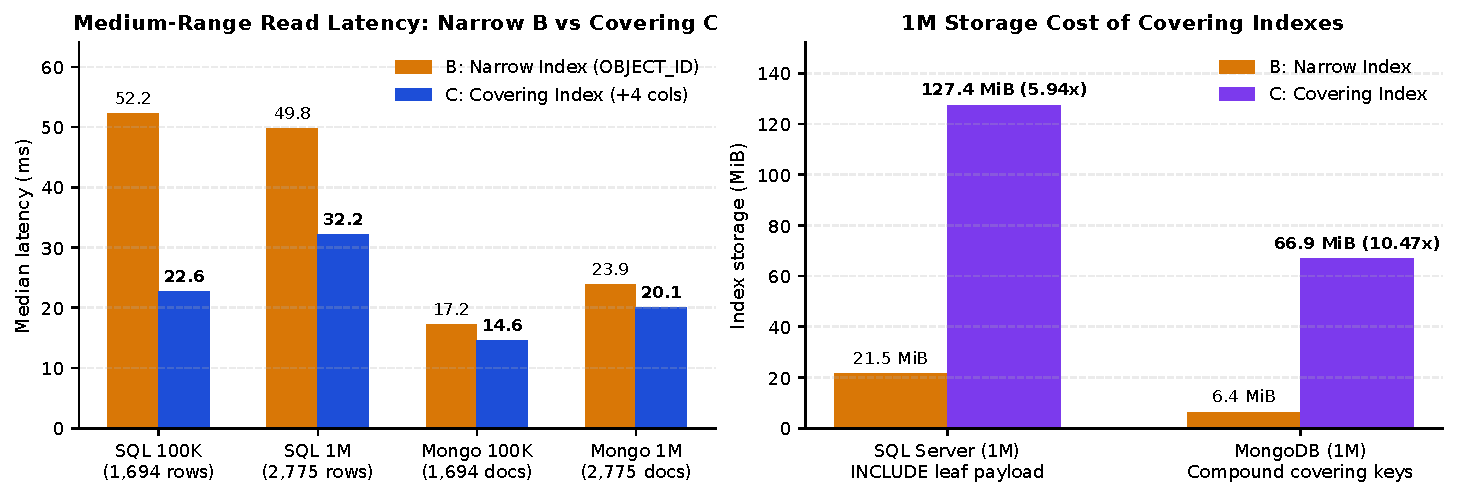
\includegraphics[width=0.94\linewidth]{figures/fig_uc3_covering.pdf}
\caption{UC3 Medium-range read latency (left) and 1M index storage cost (right). Covering Index C speeds up medium range scans by eliminating base-table lookups, but increases index size by $5.94\times$ to $10.47\times$.}
\label{fig:uc3}
\end{figure}

\ReportBlock{Why These Results Occurred}
In every single execution plan for Config C (6 in SQL Server, 6 in MongoDB), base-table lookups were completely eliminated: SQL Server plans ran a pure \texttt{Index Seek} with no \texttt{RID Lookup}, and MongoDB plans used \texttt{PROJECTION\_COVERED} with \texttt{totalDocsExamined = 0}.
\begin{enumerate}
\item \textbf{Where Coverage Matters Most (Medium Range):} At 100K Medium ($1,694$ rows), SQL Server's optimizer saw that $1,694$ random \texttt{RID Lookup}s in Narrow Index B would cost more than reading the heap, so B fell back to a $2,730$-page \texttt{Table Scan} ($52.22$\,ms). Covering Index C needed no lookups, reading just $29$ index pages in $22.63$\,ms (\textbf{$2.31\times$ faster than B}). At 1M Medium ($2,775$ rows), SQL Server logical reads dropped from $2,785$ pages in B to $49$ pages in C (\textbf{$1.54\times$ faster}), and MongoDB improved from $23.91$\,ms to $20.12$\,ms ($1.19\times$ over B, $128.2\times$ over A).
\item \textbf{Why Coverage Does Not Always Reduce Latency on Point/Small Queries:} When a query returns only $1$ to $98$ rows from an in-memory table, Narrow Index B already finishes in under $3.5$\,ms. In MongoDB 100K Small ($98$ docs), Covering Index C was actually slower than B ($4.40$\,ms vs.\ $2.83$\,ms, $0.64\times$) and tied at 1M Small ($3.49$\,ms vs.\ $3.48$\,ms), because scanning and extracting four strings from C's much wider compound index keys cost as much CPU time as fetching $60$--$98$ cached documents.
\end{enumerate}

\ReportBlock{Index Cost and Trade-Offs}
Table~\ref{tab:uc3-tradeoff} quantifies the heavy storage cost of covering indexes. Duplicating four payload columns into the index inflates 1M index storage by \textbf{$5.94\times$ in SQL Server} ($21.46 \rightarrow 127.42$\,MiB) and \textbf{$10.47\times$ in MongoDB} ($6.39 \rightarrow 66.85$\,MiB), while reducing 1M SQL Server \texttt{INSERT} throughput by $14.7\%$ compared to Baseline A.

\begin{table}[H]
\centering\small
\caption{UC3: removing base-row lookups requires a much larger covering index.}
\label{tab:uc3-tradeoff}
\begin{tabular}{@{}l l r r r@{}}
\toprule
Engine / scale & Config & Size (MiB) & Build (ms) & Insert (rows/s)\\
\midrule
SQL 100K & B & 2.27 & 118 & 3,694\\
SQL 100K & C & 12.45 & 260 & 3,888\\
SQL 1M & B & 21.46 & 1,510 & 5,813\\
SQL 1M & C & 127.42 & 1,250 & 5,230\\
\midrule
Mongo 100K & B & 0.82 & 801 & 4,472\\
Mongo 100K & C & 6.66 & 892 & 4,077\\
Mongo 1M & B & 6.39 & 10,363 & 2,190\\
Mongo 1M & C & 66.85 & 13,702 & 2,928\\
\bottomrule
\end{tabular}
\par\smallskip\scriptsize\raggedright At 1M, C/B index size is 5.94$\times$ in SQL and 10.47$\times$ in MongoDB. Insert rates do not isolate index-maintenance cost.\par
\end{table}

\ReportBlock{Practical Verdict}
Use a \textbf{Covering Index} only for high-frequency range queries that return hundreds or thousands of rows, where eliminating random \texttt{RID Lookup} or \texttt{FETCH} jumps saves major I/O. Do \emph{not} add wide covering columns for point lookups or tiny ranges: a narrow index is already under $3.5$\,ms and avoids a $6\times$ to $10\times$ memory and disk explosion.

\FloatBarrier
\section{UC4: Full-Text and Text Search over Prose (10K News Articles)}

\ReportBlock{Experimental Setup}
Six word or phrase searches run on 10K news articles. A scans \texttt{BODY} with SQL \texttt{LIKE} or MongoDB regex; C uses SQL \texttt{CONTAINS} or MongoDB \texttt{\$text}; B is not applicable. Token search should reduce scanning, but result IDs may differ from substring search. Build, writes, and search freshness are separate costs.

\ReportBlock{Measured Results}
Because substring scans match arbitrary character sequences while full-text indexes match linguistic tokens and stems, we must check whether A and C return the \textbf{exact same document IDs} before calling any latency ratio a ``same-result speedup.'' Table~\ref{tab:uc4-read} and Figure~\ref{fig:uc4} present the results.

\begin{table}[H]
\centering\small
\caption{UC4: substring A and linguistic C; exact ID equality gates speedup claims.}
\label{tab:uc4-read}
\begin{tabular}{@{}l l r r r r c@{}}
\toprule
Engine & Search & A IDs & C IDs & A p50 & C p50 & Same IDs?\\
\midrule
SQL & election & 2,577 & 2,311 & 3,294.2 & 21.00 & No\\
SQL & climate & 326 & 324 & 3,983.5 & 17.40 & No\\
SQL & bitcoin & 7 & 6 & 3,987.0 & 14.86 & No\\
SQL & white house & 1,851 & 1,845 & 3,439.6 & 22.55 & No\\
SQL & climate change & 214 & 215 & 4,042.0 & 16.63 & No\\
SQL & stock market & 45 & 37 & 4,060.1 & 14.13 & No\\
\midrule
Mongo & election & 2,577 & 3,083 & 384.60 & 15.18 & No\\
Mongo & climate & 326 & 326 & 299.96 & 6.41 & Yes\\
Mongo & bitcoin & 7 & 7 & 197.50 & 1.83 & Yes\\
Mongo & white house & 1,851 & 1,851 & 140.53 & 42.58 & Yes\\
Mongo & climate change & 214 & 214 & 288.39 & 52.39 & Yes\\
Mongo & stock market & 45 & 45 & 419.56 & 25.55 & Yes\\
\bottomrule
\end{tabular}
\par\smallskip\scriptsize\raggedright All p50 values are milliseconds. SQL A/C ID sets differ for every query. Mongo election also differs; its five other A/C ID lists match exactly.\par
\end{table}

\begin{figure}[H]
\centering
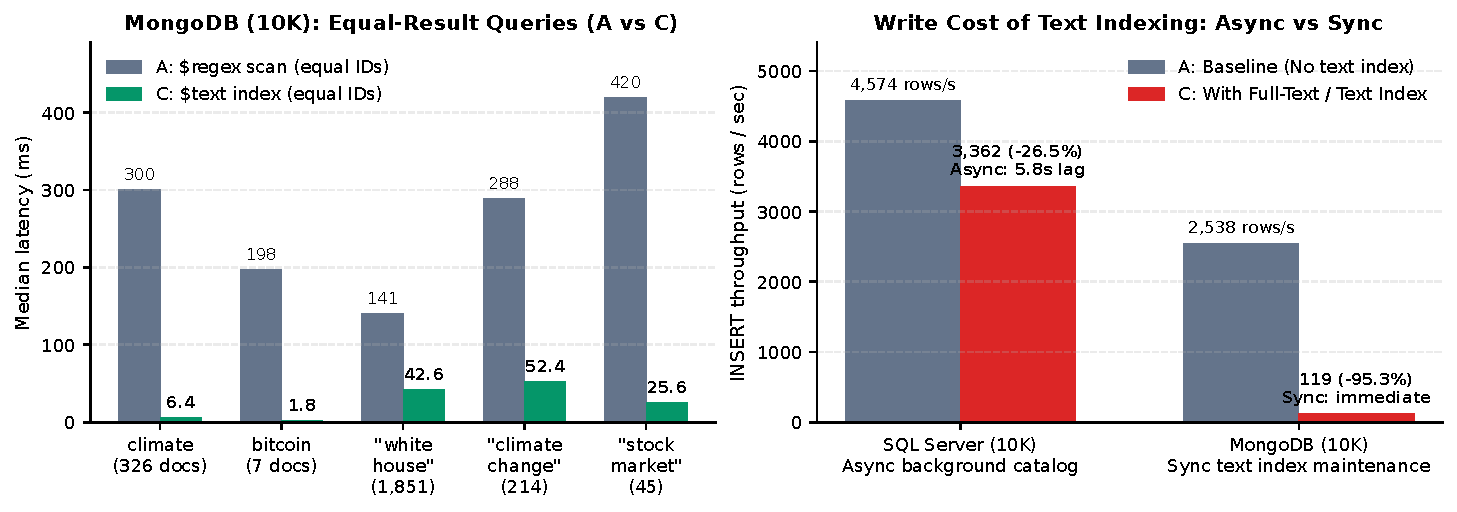
\includegraphics[width=0.94\linewidth]{figures/fig_uc4_fulltext.pdf}
\caption{UC4 (10K News) MongoDB equal-result query latencies (left) and the asynchronous vs.\ synchronous write throughput trade-off (right).}
\label{fig:uc4}
\end{figure}

\ReportBlock{Why These Results Occurred}
\begin{enumerate}
\item \textbf{Why Latency Drops Dramatically:} In SQL Server, \texttt{LIKE N'\%term\%'} scans all $7,960$ pages of the 10K table and inspects every character, taking $3.29$ to $4.06$\,seconds per query. \texttt{CONTAINS} uses the inverted index (\texttt{FulltextMatch}) and finishes in \textbf{$14.13$ to $22.55$\,ms} (reading only $69$ base pages), though we do not report a same-result speedup ratio because \texttt{LIKE} and \texttt{CONTAINS} return slightly different ID sets on all six queries. In MongoDB, on the five queries that return the \textbf{exact same IDs}, \texttt{\$text} is \textbf{$46.8\times$ to $107.8\times$ faster} on single words (\texttt{climate}, \texttt{bitcoin}) and \textbf{$3.3\times$ to $16.4\times$ faster} on exact phrases. Phrase queries are slower than single-word queries in MongoDB because the text index stores individual word stems, not multi-word phrases: for \texttt{"climate change"}, MongoDB must scan the posting lists for both \emph{climate} and \emph{change} ($3,522$ keys) and fetch $2,922$ candidate documents (\texttt{TEXT\_MATCH}) to verify that the two words appear side by side.
\item \textbf{Why \texttt{election} Returns 538 Extra Documents in MongoDB:} MongoDB's English Snowball stemmer reduces \texttt{"election"} to the root stem \texttt{"elect"}, matching articles containing \emph{elect}, \emph{elected}, or \emph{electoral} ($538$ extra documents), while missing $32$ documents where \texttt{election} was attached to another string without a word boundary.
\end{enumerate}

\ReportBlock{Index Cost and Trade-Offs}
Table~\ref{tab:uc4-tradeoff} highlights the sharpest architectural trade-off in our study:
\begin{itemize}
\item \textbf{SQL Server (Asynchronous Background Indexing):} SQL Server updates its full-text catalog in the background (\texttt{CHANGE\_TRACKING = AUTO}). As a result, \texttt{UPDATE} latency is unaffected ($3.00$\,ms vs.\ $2.99$\,ms) and \texttt{INSERT} throughput drops by only $26.5\%$, \textbf{but a newly updated article was not visible to full-text search for $5,795.4$\,ms ($5.80$\,seconds)}.
\item \textbf{MongoDB (Synchronous In-Write Indexing):} MongoDB tokenizes and updates its text index synchronously inside every write. The updated text was found at the first $21.30$\,ms poll in this probe, \textbf{but batch \texttt{INSERT} throughput collapses by $95.3\%$} (from $2,538$\,rows/s down to $119$\,rows/s, with p95 batch latency jumping to $704.9$\,ms) and \texttt{UPDATE} latency triples ($38.71 \rightarrow 115.47$\,ms).
\end{itemize}

\begin{table}[H]
\centering\small
\caption{UC4: text-index build, storage, and insert cost.}
\label{tab:uc4-tradeoff}
\begin{tabular}{@{}l l r r r r@{}}
\toprule
Engine & Configuration & Reported size & Build (s) & Insert (rows/s) & Update p50 (ms)\\
\midrule
SQL & A: PK only & 0 & 0 & 4,574 & 2.99\\
SQL & C: full-text & 13.0 & 15.20$^*$ & 3,362 & 3.00\\
Mongo & A: PK only & 0 & 0 & 2,538 & 38.71\\
Mongo & C: text & 25.19 & 11.58 & 119 & 115.47\\
\bottomrule
\end{tabular}
\par\smallskip\scriptsize\raggedright $^*$SQL size is catalog logical MB; Mongo size is index bytes divided by $2^{20}$ (MiB), so the two sizes are not directly comparable. SQL DDL returned in 63.06 ms; 15.20 s is background population. In one update probe, search visibility was observed at 5.80 s (SQL) and at the first 21.30 ms poll (Mongo); neither is a general freshness guarantee.\par
\end{table}

\ReportBlock{Practical Verdict}
Use \textbf{Full-Text / Text Indexes} for natural-language word and phrase search over articles, descriptions, or comments where scanning text takes hundreds or thousands of milliseconds. Do \emph{not} use them when you need exact arbitrary substring matching (such as partial codes or URLs), and plan carefully for SQL Server's multi-second background visibility lag or MongoDB's $95\%$ write-throughput penalty on text-heavy inserts.

\FloatBarrier
\section{UC5: Clustered Columnstore vs.\ Rowstore Heap (1M Rows, SQL Server)}

\ReportBlock{Experimental Setup}
On 1M rows in SQL Server, B is a 14-column rowstore heap and C is a clustered columnstore. The queries aggregate by \texttt{OBJECT\_TYPE} or find \texttt{ID=1} without an ID B-tree. Compressed column segments should help aggregation; the point query still has no seek path. Small writes can add delta-rowgroup work.

\ReportBlock{Measured Results}
Table~\ref{tab:uc5-read} and Figure~\ref{fig:uc5} compare Rowstore Heap B and Clustered Columnstore C at 1,000,000 rows.

\begin{table}[H]
\centering\small
\caption{UC5: SQL rowstore heap B versus clustered columnstore C.}
\label{tab:uc5-read}
\begin{tabular}{@{}l r r r r@{}}
\toprule
Query & B p50 (ms) & C p50 (ms) & B/C & C physical work\\
\midrule
Aggregation (35 groups) & 123.20 & 42.44 & 2.90$\times$ & 1,105 LOB reads; batch mode\\
Unindexed point scan & 88.81 & 3.63 & 24.49$\times$ & 776 LOB reads; still a scan\\
\bottomrule
\end{tabular}
\par\smallskip\scriptsize\raggedright B used 28,032 logical page reads on both queries. LOB reads and logical page reads count different work.\par
\end{table}

\begin{figure}[H]
\centering
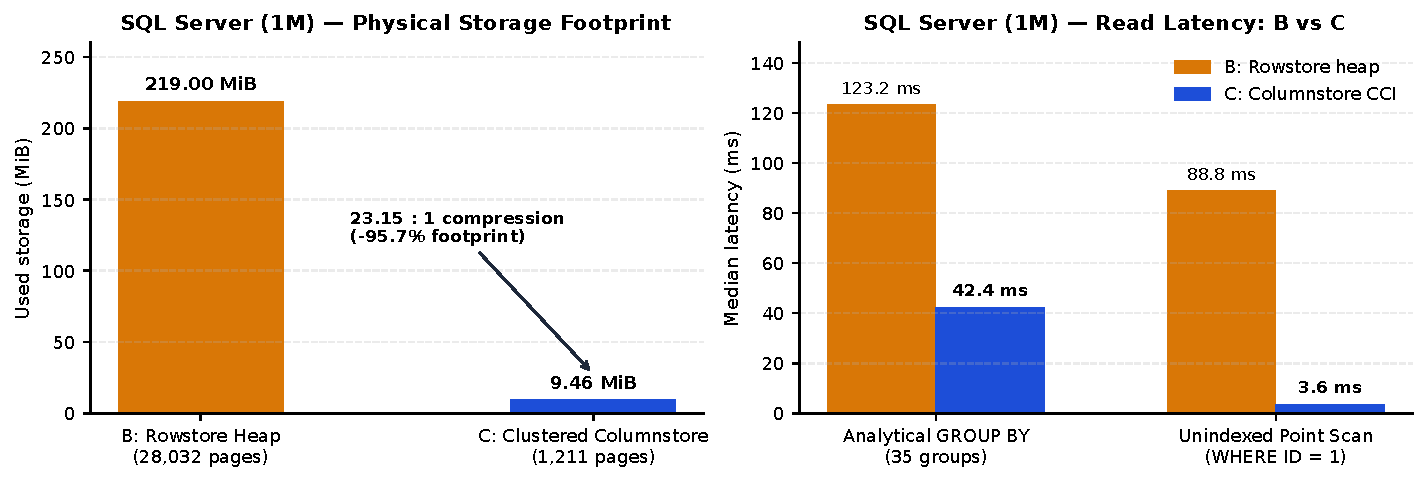
\includegraphics[width=0.94\linewidth]{figures/fig_uc5_columnstore.pdf}
\caption{UC5 (1M Rows, SQL Server) physical storage compression (left) and read latency comparison (right) between Rowstore Heap B and Clustered Columnstore C.}
\label{fig:uc5}
\end{figure}

\ReportBlock{Why These Results Occurred}
\begin{enumerate}
\item \textbf{Column Elimination (\texttt{AGG}):} Rowstore Heap B read $28,032$ logical pages from a table whose rows contain all 14 columns. C read compressed segments for the two required columns, recording $1,105$ LOB reads, and finished \textbf{$2.90\times$ faster} ($42.44$\,ms vs.\ $123.20$\,ms). The actual plans show \textbf{batch execution in both B and C}; B used batch mode on rowstore. The observed difference therefore cannot be attributed to a row-versus-batch mode switch. LOB reads and logical reads are different counters and are not a direct page-saving ratio.
\item \textbf{Why \texttt{POINT} Is Faster Here Without Being a B-Tree Seek:} On \texttt{WHERE ID = 1}, CCI C measured $3.63$\,ms versus $88.81$\,ms for Heap B. Neither copy has an ID B-tree; the actual plans show a row-mode table scan in B and a batch-mode columnstore scan in C. The counters were $28,032$ logical reads in B and $776$ LOB reads in C, which are different units. This experiment does not test C against an indexed ID seek and cannot establish columnstore as the better point-lookup design.
\end{enumerate}

\ReportBlock{Index Cost and Trade-Offs}
As shown in Table~\ref{tab:uc5-tradeoff}, CCI C compresses the 1M table from $219.00$\,MiB down to \textbf{$9.46$\,MiB ($23.15 : 1$ compression ratio)}, saving $95.68\%$ of storage, but requires $22.29$\,seconds to build. When we ran 10 small batches of 20 \texttt{INSERT}s ($200$ rows) and 10 batches of 20 \texttt{UPDATE}s ($200$ rows), small-batch \textbf{\texttt{INSERT} throughput dropped by $49.9\%$} ($13,265 \rightarrow 6,642$\,rows/s). Inspecting SQL Server's rowgroup catalog (\texttt{sys.dm\_db\_column\_store\_row\_group\_physical\_stats}) after the write test revealed the exact textbook mechanism: rowgroup 0 remained \texttt{COMPRESSED} with $1,000,000$ rows and \textbf{$200$ deleted rows} marked in its delete bitmap, while a new \texttt{OPEN} delta rowgroup (rowgroup 1) held \textbf{$400$ uncompressed rows} ($200$ inserts + $200$ updated versions).

\begin{table}[H]
\centering\small
\caption{UC5: whole-copy storage, build, and small-batch insert cost.}
\label{tab:uc5-tradeoff}
\begin{tabular}{@{}l r r r r@{}}
\toprule
Layout & Used space (MiB) & Build (s) & Insert (rows/s) & Update p50 (ms)\\
\midrule
B: rowstore heap & 219.00 & 0 & 13,265 & 154.44\\
C: clustered columnstore & 9.46 & 22.29 & 6,642 & 34.51\\
\bottomrule
\end{tabular}
\par\smallskip\scriptsize\raggedright After writes, C had one compressed 1M-row group with 200 deleted rows and one open delta rowgroup with 400 rows. The update duration includes finding rows without an ID index.\par
\end{table}

\ReportBlock{Practical Verdict}
Use a \textbf{Clustered Columnstore Index} for analytical reporting and historical tables where strong compression and scans of a few columns matter. In this run, the aggregate improved even though both layouts used batch execution. Small-batch inserts were slower; a selective point-lookup workload needs a separately evaluated B-tree access path.

\FloatBarrier
\section{UC6: Multikey vs.\ Normalized Child Index (10K Parents / 30,471 Tags)}

\ReportBlock{Experimental Setup}
At 10K parents and 30,471 tag memberships, two one-tag and two two-tag queries return parent IDs. SQL A has a child-table PK ordered by parent; SQL C adds \texttt{(TAG, PARENT\_ID)}. MongoDB A has no tag index; C adds \texttt{\{tags:1\}}. Selective tags should seek, but MongoDB may fetch candidates to check the second tag.

\ReportBlock{Measured Results}
Across all four queries, SQL Server and MongoDB returned the exact same parent ID lists. Table~\ref{tab:uc6-read} shows the read medians and the number of candidates examined.

\begin{table}[H]
\centering\small
\caption{UC6: tag membership read medians and candidate work.}
\label{tab:uc6-read}
\begin{tabularx}{\linewidth}{@{}l l r r r >{\raggedright\arraybackslash}X@{}}
\toprule
Engine & Query & A p50 & C p50 & A/C & Work in C\\
\midrule
SQL & one TABLE & 13.12 & 4.00 & 3.28$\times$ & 8 pages\\
SQL & SYS + TABLE & 16.66 & 11.69 & 1.42$\times$ & 41 pages\\
SQL & one TEMP Y & 10.51 & 0.00$^*$ & N/A & 2 pages\\
SQL & TABLE + TEMP Y & 10.85 & 2.01 & 5.39$\times$ & 10 pages\\
\midrule
Mongo & one TABLE & 18.08 & 11.58 & 1.56$\times$ & 1,247 keys and docs\\
Mongo & SYS + TABLE & 21.73 & 13.07 & 1.66$\times$ & 1,247 keys and docs\\
Mongo & one TEMP Y & 28.24 & 2.84 & 9.94$\times$ & 51 keys and docs\\
Mongo & TABLE + TEMP Y & 28.53 & 2.06 & 13.85$\times$ & 51 keys and docs; 41 matches\\
\bottomrule
\end{tabularx}
\par\smallskip\scriptsize\raggedright All p50 values are milliseconds; both baselines scanned 30,471 child rows or 10K documents. $^*$SQL 0.00 is below the timer resolution.\par
\end{table}

\ReportBlock{Why These Results Occurred}
\begin{enumerate}
\item \textbf{Why Baseline A Scans in Both Systems:} In SQL Server A, the child table's primary key is \texttt{(PARENT\_ID, TAG)}. Because \texttt{TAG} is the second column, filtering by \texttt{TAG} forces a full scan of all $30,471$ child rows ($150$ pages). Adding \texttt{IX\_UC6\_Tag\_C\_TagParent(TAG, PARENT\_ID)} in C flips the key order, reducing reads to $2$--$41$ pages ($1.42\times$ to $5.39\times$ faster).
\item \textbf{How MongoDB Executes Two-Tag \texttt{\$all} Queries on a Multikey Index:} A multikey index on \texttt{\{tags: 1\}} creates $30,471$ individual tag entries for the $10,000$ documents, but each index entry holds only \emph{one} tag string. When running \texttt{TWO\_TABLE\_TEMP\_Y} (\texttt{\$all: ["type:TABLE", "temporary:Y"]}, $41$ matches), MongoDB's \texttt{explain("executionStats")} shows that it uses \texttt{IXSCAN} on the more selective tag (\texttt{"temporary:Y"}) to find \textbf{$51$ index keys}, fetches those \textbf{$51$ candidate documents} in \texttt{FETCH}, and checks whether \texttt{"type:TABLE"} is also in their \texttt{tags} array (\textbf{$13.85\times$ speedup} over scanning all $10,000$ documents). Similarly, on \texttt{TWO\_SYS\_TABLE}, it seeks the $1,247$ \texttt{"type:TABLE"} documents and filters for \texttt{"owner:SYS"} in \texttt{FETCH} to return $1,125$ parents.
\end{enumerate}

\ReportBlock{Index Cost and Trade-Offs}
Table~\ref{tab:uc6-tradeoff} shows the storage and write costs. Because each parent document has an average of $3.05$ tags, MongoDB's multikey index must insert 3 to 5 B-tree entries per new document, reducing batch \texttt{INSERT} throughput by \textbf{$29.3\%$} ($7,451 \rightarrow 5,272$\,parents/s) and increasing tag-append (\texttt{\$addToSet}) latency by \textbf{$33.0\%$} ($27.06 \rightarrow 36.00$\,ms per 20-parent batch).

\begin{table}[H]
\centering\small
\caption{UC6: index size, build, and parent-insert throughput.}
\label{tab:uc6-tradeoff}
\begin{tabular}{@{}l l r r r r@{}}
\toprule
Engine & Configuration & Size (MiB) & Build (ms) & Insert (parents/s) & Add tag p50 (ms)\\
\midrule
SQL & A: child PK & 0 & 0 & 2,222 & 1.94\\
SQL & C: TAG, parent & 1.30 & 173.9 & 3,733 & 1.99\\
Mongo & A: no tag index & 0 & 0 & 7,451 & 27.06\\
Mongo & C: multikey & 0.17 & 211.3 & 5,272 & 36.00\\
\bottomrule
\end{tabular}
\par\smallskip\scriptsize\raggedright Add-tag p50 uses a 20-parent batch. SQL insert throughput differs from its per-batch p50 and is not interpreted as a gain from indexing.\par
\end{table}

\ReportBlock{Practical Verdict}
Use a \textbf{Multikey Index} in MongoDB or an inverted \textbf{\texttt{(TAG, PARENT\_ID)} Index} on a relational child table whenever queries filter by array elements or tags, especially when at least one queried tag is selective ($9.9\times$ to $13.9\times$ speedup in MongoDB; $3.3\times$ to $5.4\times$ in SQL Server). Keep array sizes bounded, because every additional element in a document's array multiplies the number of B-tree entries that must be maintained on writes.
\FloatBarrier
